% Chapter Template

\chapter{Problem Description and Background Research} % Main chapter title

\label{Chapter3} % Change X to a consecutive number; for referencing this chapter elsewhere, use \ref{ChapterX}

\lhead{Chapter 3. \emph{Problem Description and Background Research}} % Change X to a consecutive number; this is for the header on each page - perhaps a shortened title

%----------------------------------------------------------------------------------------

\section{Problem Description}

Medical appointment scheduling is a complex problem; patients often come with different backgrounds and personal schedules, requiring different treatment and different urgency, some even requiring support in getting to the appointments. Patients sometimes have a need to cancel their appointments or simply do not turn up, which can lead to a waste in resources if the appointment slot is not then assigned to another patient. Often, sessions can overrun, requiring more time per patient than is estimated, and so the following appointments are delayed. Clinics also reschedule appointments regularly, as new patients requiring urgent medical attention become a higher priority. This results in appointments being dynamic, often the time and date of the actual appointment is different from what was originally planned.

Dynamic scheduling leads to many issues. The problem of scheduling appointments becomes far more complex, which in turn requires more staff resources to manage the appointments.

Communication also becomes a problem, as patients need to be informed about all changes to the original schedule. Often, this results in a lower patient satisfaction and a higher chance of appointment cancellations.

These often contribute to longer waiting times and a lack of patient knowledge about their appointments, which can make no-shows and further last-minute cancellations more frequent. Often the clinic will not find a patient to take the free appointment slot, and these resources are wasted. In 2012, the Department of health announced that 1 in 10 NHS appointments are unfilled, costing the taxpayer up to £600 million a year.\cite{NHSAppsMissed}

\section{Wasted Resources}

Many resources are wasted through appointment no-shows and cancellations. Research shows that the longer a patient must wait between making the appointment and the actual appointment date, the more likely it is that they will either cancel or not turn up\cite{Gallucci}. Although we can see that there is a relationship between the length of time that a patient must wait for an appointment and the cancellation risk, it is important to understand why.

The most common reasons why patients do not show up was collected through patient questionnaires as can be seen in the figure below.

\begin{figure}[htbp]
	\centering	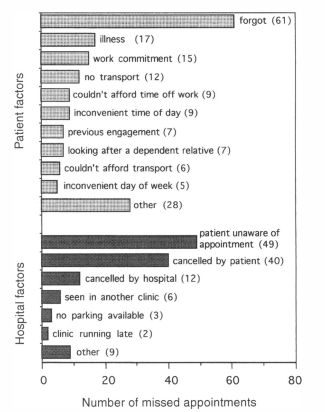
\includegraphics[width=10cm,height=10cm,keepaspectratio]{Figures/MissedAppointmentsStoneEtAl.png}
		\rule{35em}{0.5pt}
	\caption[Factors contributing to non-attendance according to a patient questionaire - \cite{Stone}]{Factors contributing to non-attendance according to a patient questionaire - \cite{Stone}}
	\label{fig:NonAttendance}
\end{figure}

This shows that the most common factor is either that the patient forgot or that they were improperly informed by the clinic.

\subsection{Patient No-Shows}

Patient no-shows (or non-attendance at outpatient clinics) are a big problem in appointment scheduling and is one of the largest contributors to wasted resources in the NHS. It is estimated  that the financial cost of missed appointments contributes to a loss of £360 million per year\cite{Stone}. Besides the financial costs, it also increases waiting times as that patient must be rescheduled for another appointment, effectively doubling the required resources per patient. 

Because the most common factor contributing to no-shows is the patient forgetting to attend the appointment, it suggests a reminder system could be used effectively to reduce these numbers. Research has shown that telephone and postal reminders can help, but have not proved to be cost effective in the past\cite{Mann}. However, through recently emerging online devices and 'smart' technology, it is possible to provide a low-cost solution to this problem.

Another factor that can encourage non-attendance can be a lack of information known about the appointment. This can introduce a level of uncertainty within the patient, such as knowledge on how to get to their appointment, or  fear about the dangerous/embarrassing factors involved in the appointment\cite{Frankel}.

Research shows that the population that miss appointments are increasingly of a young demographic. Often they fail to understand why the appointments are important, and specifically why it is important to cancel the appointment rather than just not turn up.

Patients have given several reasons for no-shows in studies and questionnaires\cite{Lacy}:

\begin{itemize}
	\item can't get time off work
	\item child-care
	\item lack of transportation or cost
	\item patient felt better or felt too worse to attend the appointment
\end{itemize}

For all these reasons, the no-show is preventable simply by increasing communication with the patient and allowing them either more information about the appointment or making it easier for them to either cancel/reschedule.

\subsection{Cancellations}

Often, clinics are required to cancel an outpatients appointment for a variety of reasons, usually due to a lack of resources such as staff or equipment.

Staff time is then wasted getting contact information for the patient and informing them of the cancellation. Time must also be spent corresponding with the patient and agreeing on a suitable replacement appointment.

If cancellations 'occur at the last minute', often the patient is not informed until they reach the hospital. This is often due to the clinic not wanting to bother wasting resources reaching the patient when it is unlikely that they will get a hold of them (the patient may already be in transit or indisposed). This leads to a lower overall user satisfaction as the patient wastes a trip to the hospital, only to find that they no longer have an appointment.

Although cancellations are not ideal, they are better than no-shows in that it is possible for the appointment to be offered to another patient. In some cases however, this is not attempted due to it being too costly and the additional complexity involved in the scheduling process.

By increasing communication with patients through emerging smart technology, it may be possible for these appointments to be quickly rescheduled whilst avoiding the additional costs, even for 'last-minute' cancellations.

\subsection{Managing Appointments}

Managing appointments is costly and a large proportion of the work is carried out by individual staff members, rather than an automated system. Several issues arise with this process:

\begin{itemize}
	\item Appointments can only be managed within office hours (typically 9am - 5pm), however this depends on the clinic
	\item Patients can only make appointments over the phone and frequently have to queue to speak to a staff member
	\item Large proportions of staff members must be allocated to the appointments procedure which could be allocated elsewhere
	\item State of the system means that it is hard to analyse and therefore adapt to high demand
	
\end{itemize}

When making appointments, the patient is required to do so either in person or over the phone. This can only occur within office hours, which can conflict with the patients career or personal schedule, leading to a lower user satisfaction. Often patients will have to queue in order to speak to a staff member. When the patient is finally connected, there isn't time for the patient to explain their personal schedule and discuss conflicts, resulting in less user choice and flexibility.

The appointment system in many areas is also very labour-intensive, carried out by individual receptionists using spreadsheets and paper based systems\cite{ApointProcWebsite}. This means that it is often very hard to analyse capacity and demand, identifying bottlenecks or methods to improve them and also makes it very hard to integrate with interactive technology such as smart phone devices and online appointments. Whilst some online systems do exist\cite{C&BWebsite}, they are time consuming, have poor functionality and tend to be only available on few devices\cite{C&BFailure}. 

These problems can be improved by creating an interactive online system that works on many devices. It could not replace the current system entirely, because not all patients will have internet access or smart-devices, but it would provide benefits to patients with internet access such as:

\begin{itemize}
	\item Easier accessibility to making appointments
	\item Possibly offer more appointment flexibility to the patient
	\item More information about the appointment
	\item Relieve demand on the staff that manage the system
	\item More analysis of appointment trends and offer insights into improvement
\end{itemize}

\section{Patient Satisfaction and Experience}

Maintaining a high patient satisfaction is the primary goal in appointment scheduling, ultimately because keeping the patients happy leads to less cancellations and less no-shows. This is not an easy task because the demand on the healthcare system is so great, and it is typically faced with many challenges.

\subsection{Patient Requirements}

Patients are given a level of responsibility that some may not be used to. For a general outpatient appointment, the NHS requires the patient to do a number of tasks to prepare for the appointment \cite{OutpatientApointWebsite}:

\begin{itemize}
  \item may be required not to eat/drink before the appointment
  \item may be required to bring samples of urine/stool or medicines
  \item may need to bring previous test results
  \item may need to take certain medicines at a certain time period prior to the appointment
  \item should bring maps and other information required for getting to their appointment
\end{itemize}

It has been seen that in previous research conducted on day surgery outpatients, the most likely cause of preventable appointment cancellations (5\% of day surgery appointments) was due to inadequate preparation \cite{Macarthur}. This shows that a large amount of patient cancellations occur simply because patients are expected to find out information about their appointment, transport options and other relevant factors.

\subsection{Waiting times}

Another factor that lowers patient satisfaction are waiting times that can occur when the schedule is either running late due to overrunning appointments, or when patients are grouped into time slots.

Patients are frequently grouped together into time slots to simplify the scheduling process (i.e the clinic will expect to have 10 appointments in one hour, so they ask all 10 patients to come at the same time and the appointments occur on a first come first serve basis).

Research suggests that because patients spend increasingly lengthy amounts of time waiting in the clinic for their appointment to start, they feel increasingly amounts of disrespect \cite{Lacy}. This is due to patients being 'left in the dark', with no indication on why their appointment is delayed and why they have to wait.

Through on-line applications and smart devices, we can inform patients about information related to their appointments, any disruptions in the regular service (waiting delays) and a more interactive system that would make the patient feel less disrespect. We will also be able to offer sooner appointments to patients as cancellations occur, which should reduce the waiting times overall.

We can also provide transport information, reminders on when they have to leave and any perquisite requirements that the patient must undertake before leaving for their appointment (such as take medication or bring test results), reducing the likelihood of cancellations and no-shows as the patient is better prepared..

\subsection{Patient Participation}

Patient participation is no longer just a goal set by medical commissioners, but a legal obligation. The Health and Social Care Act 2012\cite{HSCA2012} introduced legislation that enables patients(and carers) to participate in the planning, managing and making decisions
about their care and treatment.

The aim of this project targets this participation, engaging patients to have more control and access over their medical care. This system also has the ability to deliver personalised care plans to patients, which will increase the overall patient satisfaction.

Although this system does require patients to have access to the internet and know how to use it, patients without internet in today's world is an increasingly small demographic. The NHS are also launching a program to help disadvantaged people learn how to access the internet and use medical services \cite{timKelsey}, to try and combat these issues. 

%----------------------------------------------------------------------------------------

\section{Choose and Book - An existing online medical appointment service}

An NHS service 'Choose and Book' was launched in 2006, aimed at providing patients with more choice through online appointments\cite{Walford}.

This system is similar to the project area in that it allows patients to create online outpatient appointments, having a choice over which clinic they go to and when they the appointment is booked for.

However, an independent survey of patient's experience using the service in 2008 showed that patients did not receive the degree of choice that the service was designed to deliver\cite{Green}. It has also been widely criticised as being time consuming, over complicated and . An article in 2012\cite{C&BFailure} shows that the system's popularity is diminishing.

Besides the clear flaws in the system such as ease of use and failing to offer more choice, it also fails to target significant areas of the problem description, such as electronic reminders, recycling unused appointments and general appointment information.

%----------------------------------------------------------------------------------------

\section{Conclusion}

Attempts have been made in the past to simplify the appointment management process and take it online, however they fail to hit all of the objectives simply because the platforms were not ready. As smart-devices and their many applications are becoming increasingly popular, it opens up a new gateway to communicate directly with patients and receive quick response times. This makes it much easier to create a dynamic appointment schedule whilst maintaining a high user satisfaction level.

This project will therefore focus on improving the communication and interactivity between patients and the appointment scheduling system; so that more information is available to the patient, there is more chance of reusing free appointment slots, and less staff resources are used in managing appointments so they can be allocated to other areas.

The project will also look at making the appointment creation and rescheduling process easier for both patients and staff, requiring less management resources and offering more platform choices and flexibility.